\chapter{\sffamily Managing a rugby match}

{\bfseries\sffamily Concept.} Building a toy model simulation of a rugby match whose outcome can be manipulated through correctly-timed player substitutions and game management decisions. The dexetera state manipulation framework we have built around the stochadex can meet these requirements, and a dashboard can be created for user interaction. All this combines together to make a simple dashboard game, which we call: `trywizard'. For the mathematically-inclined, this chapter will motivate the construction of a specific modelling framework for rugby match simulation. For the programmers, the public Git repository for the code described in this chapter can be found here: \href{https://github.com/umbralcalc/trywizard}{https://github.com/umbralcalc/trywizard}.

\section{\sffamily Designing the event simulation engine}

Since the basic state manipulation framework and simulation engine will run using \href{https://github.com/umbralcalc/dexetera}{dexetera}, the mathematical novelties in this project are all in the design of the rugby match model itself. And, as ever, we're not especially keen on spending a lot of time doing detailed data analysis to come up with the most realistic values for the parameters that are dreamed up here. Even though this would also be interesting.\footnote{One could do this data analysis, for instance, by scraping player-level performance data from one of the excellent websites that collect live commentary data such as \href{https://www.rugbypass.com/}{rugbypass.com} or \href{https://www.espn.co.uk/rugby/}{espn.co.uk/rugby}.}

Let's begin by specifying an appropriate event space to live in when simulating a rugby match. It is important at this level that events are defined in quite broadly applicable terms, as it will define the state space available to our stochastic sampler and hence the simulated game will never be allowed to exist outside of it. It seems reasonable to characterise a rugby union match by the following set of events: Penalty, Free Kick (the punitive events); Penalty Goal, Drop Goal, Try (the scoring events); Kick Phase, Run Phase, Knock-on, Scrum, Lineout, Maul and Ruck (the general play events). Using this set of events, in Fig.~\ref{fig:event-graph} we have summarised our approach to match state transitions into a single event graph. In order to capture the fully detailed range of events that are possible in a real-world match, we've needed to be a little imaginative in how we define the kinds of state transitions which occur. In other words; it's fair to say that our simplified model here represents just a subset of events that a real rugby match could generate.

\begin{figure}[h]
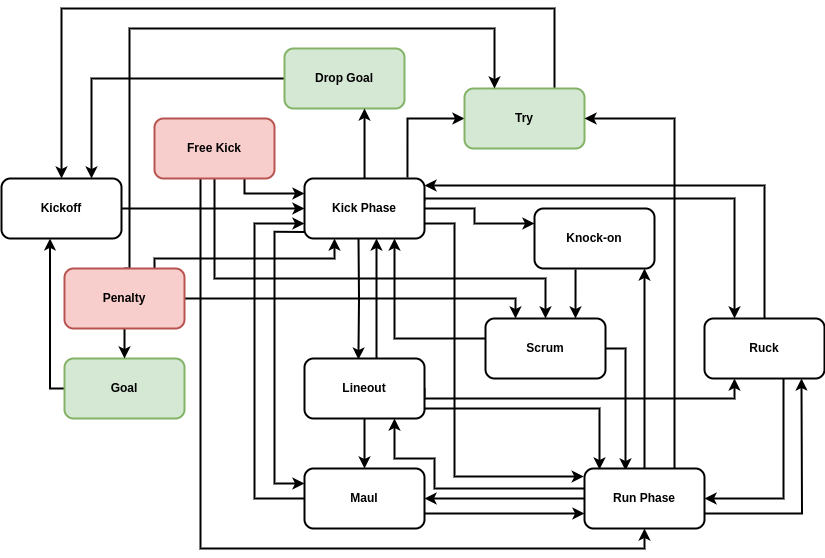
\includegraphics[width=14cm]{images/trywizard-event-graph.drawio.png}
\caption{Simplified event graph of a rugby union match.}
\label{fig:event-graph}
\end{figure}

In addition to occupying some state in the event graph, the state of a rugby match must also include a binary `possession' element which encodes which team has the ball at any moment. We should also include the 2-dimensional pitch location of the ball as an element of the match state in order to get a better sense of how likely some state transitions are, e.g., when playing on the edge of the pitch near the touchline it's clearly more likely that a Run Phase is going to result in a lineout than if the state is currently in the centre of the pitch. To add even more detail, we will include states for each playing position on each side which encode: the playing abilities of each player, their fatigue status and their substitution status. The latter of these encodes whether or not the player has been injured or yellow/red-carded during the course of a game and should also enable management strategies to become more nuanced.

Since a rugby match exists in continuous time, it is natural to choose a continuous-time event-based simulation model for our game engine. As we have discussed in previous chapters already, this means we will be characterising transition probabilities of the event graph in Fig.~\ref{fig:event-graph} by ratios of event rates in time. Recalling our notation in previous chapters, if we consider the current state vector of the match $X_{\sf t}$, we can start by assigning each transition $a\rightarrow b$ on the event graph an associated rate of occurance $\lambda_{a\rightarrow b} (X_{\sf t}, {\sf t})$ which is defined in units of continuous time, e.g., seconds. In addition to the transitions displayed on the graph, we can add a `possession change transition'; where the possession of the ball in play moves to the opposing team. This transition may occur while the match is also in any of the white-coloured states on the graph and let's assign this a time and state-dependent expected rate of occurance $\lambda_{\rm pos}(X_{\sf t}, {\sf t})$.

Based on our dicussion above, an appropriate encoding for the overall game state at timestep index ${\sf t}$ could be a state vector $X_{{\sf t}}$ whose elements are
%%
\begin{align}
X^0_{{\sf t}}&=\begin{cases} 0 & \text{Match State} = \text{Penalty}\\ 1 & \text{Match State} = \text{Free Kick} \\ \dots & \end{cases} \\
X^1_{{\sf t}}&=\begin{cases} 0 & \text{Possession} = \text{Home Team}\\ 1 & \text{Possession} = \text{Away Team} \end{cases} \,.
\end{align}
%%
But how does this overall game state connect to the event rates? The probabilistic answer is quite straightforward; if the probability of the match state being $X^0_{{\sf t}}=a$ at timestep ${\sf t}$ is written as $P^0_{{\sf t}}(a)$, then the probability of $X^0_{{\sf t}+1}=b$ in the following timestep is
%%
\begin{align}
P^0_{{\sf t}+1}(b) = \frac{\lambda_{a\rightarrow b} (X_{\sf t}, {\sf t})P^0_{{\sf t}}(a)}{\sum_{\forall b}\lambda_{a\rightarrow b} (X_{\sf t}, {\sf t})P^0_{{\sf t}}(a)} \label{eq:match-state-transition-probs}\,,
\end{align}
%%
where the $\forall b$ in the summation indicates that all the available transitions from $a$ (including the one where no transition happens at all) should be summed over.

Before we move on to other details, it's quite important to recognise that because our process is defined in continuous time, the event rates may well vary continuously (this will be especially true when we talk about, e.g., player fatigue). Hence, Eq.~(\ref{eq:match-state-transition-probs}) is only an \emph{approximation} of the true underlying dynamics that we are trying to simulate --- and this approximation will only be accurate if the increments in continuous time $\delta t({\sf t})$ are small for each timestep. The reader may recall that we discussed this same issue from the point of view of simulating time-inhomogeneous Poisson processes when we were building the stochadex.

\begin{itemize}
\item{Move on to talk about how to connect player states and abilities to the event rates.}
\end{itemize}

\section{\sffamily Deciding on gameplay actions}


\begin{itemize}
\item{Need to start thinking here about the fundamental dexetera formalism before fleshing this bit out.}
\end{itemize}

\section{\sffamily Writing the game itself}

\begin{itemize}
\item{Show which stochadex/dexetera methods were called and how they were used to simulate the game.}
\item{Give a summary of how the dashboard backend works (diagram would help) and how this connects up to the streamlit frontend via protobuf messages.}
\end{itemize}